\documentclass[aspectratio=169,11pt]{beamer}

% ── Packages ──────────────────────────────────────────────────────────────────
\usepackage{graphicx}
\usepackage{booktabs}
\usepackage{array}
\usepackage[T1]{fontenc}
\usepackage{lmodern}
\usepackage{xcolor}
\usepackage{tikz}
\usetikzlibrary{calc, positioning}
\usepackage{amsmath}
\usepackage{hyperref}
\usepackage{siunitx}
\usepackage{colortbl}
\usepackage{pgfplots}
\pgfplotsset{compat=1.18}

% ── Colour Palette ────────────────────────────────────────────────────────────
\definecolor{DeepNavy}{HTML}{2E4057}
\definecolor{Teal}{HTML}{048A81}
\definecolor{WarmOrange}{HTML}{E85D04}
\definecolor{SoftPurple}{HTML}{9D4EDD}
\definecolor{WarmGray}{HTML}{8A8A8A}
\definecolor{LightGray}{HTML}{F2F2F2}
\definecolor{Cream}{HTML}{FFFDF7}
\definecolor{DeepRed}{HTML}{C1121F}
\definecolor{Gold}{HTML}{D4A017}

% ── Theme Setup ───────────────────────────────────────────────────────────────
\usetheme{default}
\setbeamertemplate{navigation symbols}{}
\setbeamertemplate{headline}{}
\setbeamercolor{background canvas}{bg=Cream}
\setbeamercolor{frametitle}{fg=DeepNavy,bg=Cream}
\setbeamerfont{frametitle}{series=\bfseries,size=\large}

\setbeamertemplate{frametitle}{%
  \vspace*{0.3em}%
  \insertframetitle%
  \ifx\insertframesubtitle\empty\else
    \\[0.1em]{\footnotesize\color{WarmGray}\parbox{\textwidth}{\insertframesubtitle}}%
  \fi
  \par\vspace*{0.15em}%
  \textcolor{Teal}{\rule{\textwidth}{0.5pt}}%
}

\setbeamertemplate{footline}{%
  \hfill{\color{WarmGray}\tiny\insertframenumber\hspace{0.5em}}%
  \vspace{0.3em}%
}

\setbeamercolor{itemize item}{fg=Teal}
\setbeamercolor{itemize subitem}{fg=WarmOrange}
\setbeamertemplate{itemize item}{\small\raisebox{0.15ex}{\textbullet}}
\setbeamertemplate{itemize subitem}{\scriptsize\raisebox{0.15ex}{\textbullet}}

% ── Custom Macros ─────────────────────────────────────────────────────────────
\newcommand{\emphcolor}[1]{{\color{WarmOrange}\textbf{#1}}}
\newcommand{\tealtext}[1]{{\color{Teal}#1}}
\newcommand{\navytext}[1]{{\color{DeepNavy}#1}}
\newcommand{\graytext}[1]{{\color{WarmGray}#1}}

\newcommand{\transitionslide}[2]{%
  \begingroup
  \setbeamercolor{background canvas}{bg=DeepNavy}
  \setbeamertemplate{footline}{}
  \begin{frame}[plain]
    
\begin{tikzpicture}[overlay]
      \draw[Teal, opacity=0.3, line width=8pt]
        (-1,-1) -- ++(20,0) -- ++(0,12) -- cycle;
    \end{tikzpicture}
    \vspace{1.8cm}
    \hspace{0.8cm}%
    {\color{white}\bfseries\LARGE\parbox{13cm}{#1}}\\[0.6em]
    \hspace{0.8cm}%
    {\color{Teal}\normalsize\parbox{13cm}{#2}}
  \end{frame}%
  \endgroup
}

% ── Shared TikZ channel-diagram style ─────────────────────────────────────────
% box: default outcome node
% coldbox / heatbox: cause nodes

% ── Document ──────────────────────────────────────────────────────────────────
\begin{document}

% ━━━━━━━━━━━━━━━━━━━━━━━━━━━━━━━━━━━━━━━━━━━━━━━━━━━━━━━━━━━━━━━━━━━━━━━━━━━
% Slide 1 — Title
% ━━━━━━━━━━━━━━━━━━━━━━━━━━━━━━━━━━━━━━━━━━━━━━━━━━━━━━━━━━━━━━━━━━━━━━━━━━━
\begingroup
\setbeamercolor{background canvas}{bg=DeepNavy}
\setbeamertemplate{footline}{}
\begin{frame}[plain]
  \begin{tikzpicture}[overlay]
    \node[text=Teal, opacity=0.12, font=\fontsize{140}{140}\selectfont]
      at (10, 2.5) {\(\sim\)};
  \end{tikzpicture}
  \vspace{0.9cm}
  \hspace{0.6cm}%
  {\color{white}\bfseries\fontsize{22}{28}\selectfont
    \parbox{13cm}{Climate Shocks, Health Finance,\\and Economic Outcomes}}
  \par\vspace{0.45em}
  \hspace{0.6cm}%
  {\color{WarmOrange}\rule{12cm}{2pt}}
  \par\vspace{0.45em}
  \hspace{0.6cm}%
  {\color{Teal}\normalsize County-Level Evidence from the United States, 2011--2023}
  \par\vspace{0.35em}
  \hspace{0.6cm}%
  {\color{WarmGray}\small Seminar Presentation \(\cdot\) April 2026}
\end{frame}
\endgroup

% ━━━━━━━━━━━━━━━━━━━━━━━━━━━━━━━━━━━━━━━━━━━━━━━━━━━━━━━━━━━━━━━━━━━━━━━━━━━
% Slide 2 — The Gap
% ━━━━━━━━━━━━━━━━━━━━━━━━━━━━━━━━━━━━━━━━━━━━━━━━━━━━━━━━━━━━━━━━━━━━━━━━━━━
\begin{frame}[shrink=18]{Climate Science Has Cracked Mortality. Health Finance Is the Blind Spot.}
  \framesubtitle{The economic burden of climate on healthcare costs and household debt is largely unmeasured}
  \begin{columns}[T]
    \begin{column}{0.47\textwidth}
      \textbf{\tealtext{What we know well}}\\[0.2em]
      \footnotesize
      \begin{itemize}\itemsep0.18em
        \item Extreme heat, cold, and drought raise \emphcolor{mortality} — robust evidence across many countries
        \item Air pollution (PM$_{2.5}$, ozone) shortens lives and raises hospitalisation rates
        \item Climate models project these risks will intensify
      \end{itemize}
      \vspace{0.3em}
      \textbf{\tealtext{What we don't know}}\\[0.2em]
      \begin{itemize}\itemsep0.18em
        \item Does surviving a climate shock leave households \emphcolor{financially damaged}?
        \item Do insurers and hospitals \emphcolor{absorb or pass on} those costs?
        \item Does climate volatility — not just severity — matter for \emphcolor{health finance}?
      \end{itemize}
    \end{column}
    \begin{column}{0.47\textwidth}
      \textbf{\tealtext{Why this matters for adaptation}}\\[0.2em]
      \footnotesize
      \begin{itemize}\itemsep0.18em
        \item Adaptation policy that targets mortality alone may \emphcolor{miss the majority of the economic burden}
        \item Medical debt and insurance premiums are \emphcolor{regressive}: low-income households bear disproportionate shares
        \item Hospital bad debt signals coverage collapse under climate stress — an early warning for \emphcolor{system fragility}
        \item Evidence is needed at the \emphcolor{county scale} where adaptation decisions are made
      \end{itemize}
      \vspace{0.3em}
      \graytext{\scriptsize This paper: first systematic county-level evidence linking climate shocks to health finance outcomes across the U.S., 2011--2023.}
    \end{column}
  \end{columns}
\end{frame}

% ━━━━━━━━━━━━━━━━━━━━━━━━━━━━━━━━━━━━━━━━━━━━━━━━━━━━━━━━━━━━━━━━━━━━━━━━━━━
% Slide 3 — Transmission Mechanism
% ━━━━━━━━━━━━━━━━━━━━━━━━━━━━━━━━━━━━━━━━━━━━━━━━━━━━━━━━━━━━━━━━━━━━━━━━━━━
\begin{frame}{How Climate Shocks Reach Your Wallet}
  \framesubtitle{The transmission chain from weather event to household financial damage}
  \begin{center}
  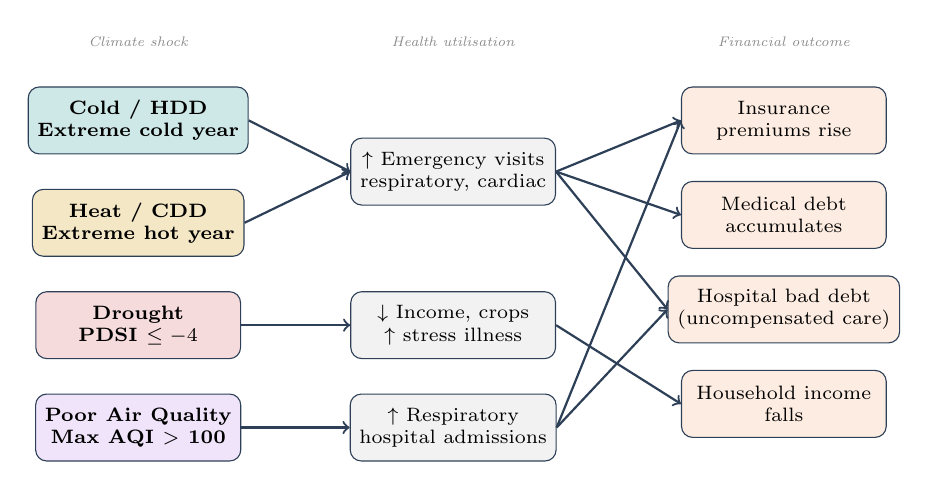
\begin{tikzpicture}[
    node distance = 0.5cm and 1.4cm,
    box/.style={draw=DeepNavy, rounded corners=4pt, fill=LightGray,
                minimum width=2.6cm, minimum height=0.85cm,
                align=center, font=\scriptsize},
    cause/.style={draw=DeepNavy, rounded corners=4pt,
                  minimum width=2.6cm, minimum height=0.85cm,
                  align=center, font=\scriptsize\bfseries},
    arr/.style={->, thick, DeepNavy},
    lab/.style={font=\tiny\itshape, text=WarmGray}
  ]
    % Column 1: shocks
    \node[cause, fill=Teal!20]   (cold)   at (0, 1.2)  {Cold / HDD\\Extreme cold year};
    \node[cause, fill=Gold!25]   (heat)   at (0,-0.1)  {Heat / CDD\\Extreme hot year};
    \node[cause, fill=DeepRed!15](drought)at (0,-1.4)  {Drought\\PDSI $\leq -4$};
    \node[cause, fill=SoftPurple!15](aqi) at (0,-2.7)  {Poor Air Quality\\Max AQI $>$ 100};

    % Column 2: utilisation
    \node[box] (util1) at (4.0, 0.55) {$\uparrow$ Emergency visits\\respiratory, cardiac};
    \node[box] (util2) at (4.0,-1.4)  {$\downarrow$ Income, crops\\$\uparrow$ stress illness};
    \node[box] (util3) at (4.0,-2.7)  {$\uparrow$ Respiratory\\hospital admissions};

    % Column 3: finance
    \node[box, fill=WarmOrange!12] (prem)  at (8.2, 1.2)  {Insurance\\premiums rise};
    \node[box, fill=WarmOrange!12] (debt)  at (8.2, 0.0)  {Medical debt\\accumulates};
    \node[box, fill=WarmOrange!12] (bad)   at (8.2,-1.2)  {Hospital bad debt\\(uncompensated care)};
    \node[box, fill=WarmOrange!12] (inc)   at (8.2,-2.4)  {Household income\\falls};

    % Arrows: shocks -> utilisation
    \draw[arr] (cold.east)    -- (util1.west);
    \draw[arr] (heat.east)    -- (util1.west);
    \draw[arr] (drought.east) -- (util2.west);
    \draw[arr] (aqi.east)     -- (util3.west);

    % Arrows: utilisation -> finance
    \draw[arr] (util1.east) -- (prem.west);
    \draw[arr] (util1.east) -- (debt.west);
    \draw[arr] (util1.east) -- (bad.west);
    \draw[arr] (util2.east) -- (inc.west);
    \draw[arr] (util3.east) -- (bad.west);
    \draw[arr] (util3.east) -- (prem.west);

    % Column labels
    \node[lab] at (0,   2.2) {Climate shock};
    \node[lab] at (4.0, 2.2) {Health utilisation};
    \node[lab] at (8.2, 2.2) {Financial outcome};
  \end{tikzpicture}
  \end{center}
  \vspace{-0.3em}
  \graytext{\scriptsize This paper measures the \emphcolor{right-hand column} directly using county panel data, bypassing utilisation data which are noisy and inconsistently reported.}
\end{frame}

% ━━━━━━━━━━━━━━━━━━━━━━━━━━━━━━━━━━━━━━━━━━━━━━━━━━━━━━━━━━━━━━━━━━━━━━━━━━━
% Slide 4 — Outcome Glossary
% ━━━━━━━━━━━━━━━━━━━━━━━━━━━━━━━━━━━━━━━━━━━━━━━━━━━━━━━━━━━━━━━━━━━━━━━━━━━
\begin{frame}[shrink=25]{What Are We Measuring? A Field Guide to Health Finance Outcomes}
  \framesubtitle{Plain-English definitions; all dollar values in \$2023}
  \footnotesize
  \renewcommand{\arraystretch}{1.55}
  \begin{tabular}{@{}>{\bfseries\color{DeepNavy}\raggedright\arraybackslash}p{0.23\linewidth}%
                     >{\raggedright\arraybackslash}p{0.44\linewidth}%
                     >{\raggedright\arraybackslash}p{0.27\linewidth}@{}}
    \rowcolor{DeepNavy}
    \textcolor{white}{Outcome} & \textcolor{white}{What it measures} & \textcolor{white}{Scale / context} \\
    \rowcolor{Teal!10}
    Benchmark Silver Premium &
      Monthly cost of the mid-tier ACA marketplace plan in a county's rating area. Insurers set this annually based on expected claims. &
      $\sim$\$400--700/month nationally; $+\$28$ = $\sim$4--7\% increase \\
    Medical Debt Share &
      Fraction of county residents with medical debt in collections, from credit bureau records (Urban Institute). &
      National mean $\sim$13\%; $+1$ pp = $\sim$8\% relative rise \\
    \rowcolor{Teal!10}
    Medical Debt Median &
      Median balance owed among those with medical debt in collections. &
      National median $\sim$\$690; $+\$30$ $\approx$ 4\% increase \\
    Hospital Bad Debt per Capita &
      Uncompensated care written off by hospitals after billing failure (not charity care). Signals patients unable to pay even after treatment. &
      Mean $\sim$\$120/capita; $+\$5$ $\approx$ 4\% increase \\
    \rowcolor{Teal!10}
    Medicaid / Medicare per Enrollee &
      Annual public payer spending per enrolled beneficiary. Falls can indicate access barriers, not just lower need. &
      Medicare $\sim$\$12,000/yr; Medicaid $\sim$\$8,000/yr \\
    Median HH Income / PCPI &
      County median household income (ACS) and BEA per-capita personal income. Both inflation-adjusted. &
      U.S.\ median HH income $\sim$\$75,000 in 2023 \\
  \end{tabular}
\end{frame}

% ━━━━━━━━━━━━━━━━━━━━━━━━━━━━━━━━━━━━━━━━━━━━━━━━━━━━━━━━━━━━━━━━━━━━━━━━━━━
% Slide 5 — Data Coverage
% ━━━━━━━━━━━━━━━━━━━━━━━━━━━━━━━━━━━━━━━━━━━━━━━━━━━━━━━━━━━━━━━━━━━━━━━━━━━
\begin{frame}{Data: Linking Climate Records to Health Finance at County Level}
  \framesubtitle{Panel: 2011--2023; $\sim$3,155 U.S.\ counties; state panel: 51 states $\times$ 13 years}
  \begin{columns}[T]
    \begin{column}{0.47\textwidth}
      \textbf{\tealtext{Climate \& Environment}}\\[0.2em]
      \scriptsize
      \begin{tabular}{@{}>{\raggedright\arraybackslash}p{0.58\linewidth}>{\raggedright\arraybackslash}p{0.34\linewidth}@{}}
        \toprule
        Variable & Source \\
        \midrule
        Annual mean temp, HDD, CDD & NOAA/NCEI \\
        Palmer Drought Severity Index & NOAA/NCEI \\
        Annual AQI (median, max) & EPA \\
        \bottomrule
      \end{tabular}
      \vspace{0.4em}
      \textbf{\tealtext{Health Finance}}\\[0.2em]
      \begin{tabular}{@{}>{\raggedright\arraybackslash}p{0.58\linewidth}>{\raggedright\arraybackslash}p{0.34\linewidth}@{}}
        \toprule
        Variable & Source \\
        \midrule
        ACA marketplace premiums & HIX Compare \\
        County medical debt & Urban Institute \\
        Hospital bad / charity debt & NASHP HCT \\
        Employer insurance contrib. & AHRQ MEPS-IC \\
        Medicaid / Medicare spending & CMS NHE \\
        \bottomrule
      \end{tabular}
    \end{column}
    \begin{column}{0.47\textwidth}
      \textbf{\tealtext{Economy \& Household}}\\[0.2em]
      \scriptsize
      \begin{tabular}{@{}>{\raggedright\arraybackslash}p{0.58\linewidth}>{\raggedright\arraybackslash}p{0.34\linewidth}@{}}
        \toprule
        Variable & Source \\
        \midrule
        Median HH income & ACS 5-yr \\
        Civilian employment & ACS 5-yr \\
        Per-capita personal income & BEA CAINC1 \\
        CPI (inflation adjustment) & FRED \\
        \bottomrule
      \end{tabular}
      \vspace{0.4em}
      \textbf{\tealtext{Key features}}\\[0.2em]
      \begin{itemize}\itemsep0.14em
        \item Climate z-scores anchored to \emphcolor{1990--2000 baseline} — shocks measured against pre-warming reference
        \item CDD/HDD thresholds: \emphcolor{national 80th percentile} — captures objectively extreme years, not just ``warm for that county''
        \item All dollar outcomes \emphcolor{inflation-adjusted to 2023}
        \item State-level cluster SEs account for \emphcolor{within-state spatial correlation}
      \end{itemize}
    \end{column}
  \end{columns}
\end{frame}

% ━━━━━━━━━━━━━━━━━━━━━━━━━━━━━━━━━━━━━━━━━━━━━━━━━━━━━━━━━━━━━━━━━━━━━━━━━━━
% Slide — Summary Statistics: Climate Stress Over Time
% ━━━━━━━━━━━━━━━━━━━━━━━━━━━━━━━━━━━━━━━━━━━━━━━━━━━━━━━━━━━━━━━━━━━━━━━━━━━
\begin{frame}{Climate Stress Is Volatile, Not Trending}
  \framesubtitle{County-level shock exposure, 2011--2023; PW = population-weighted, UW = unweighted}
  \begin{columns}[T]
    \begin{column}{0.52\textwidth}
      \centering
      \textbf{\tealtext{\small Panel A: Shock Prevalence (\% of U.S.\ pop., PW)}}\\[0.2em]
      \begin{tikzpicture}
        \begin{axis}[
          width=\linewidth,
          height=0.65\textheight,
          xmin=2011, xmax=2023,
          ymin=0, ymax=82,
          xtick={2011,2013,2015,2017,2019,2021,2023},
          xticklabel style={rotate=45, anchor=east, font=\tiny,
                             /pgf/number format/1000 sep={}},
          ytick={0,20,40,60,80},
          yticklabel={\pgfmathprintnumber{\tick}\%},
          grid=major,
          grid style={line width=0.3pt, draw=gray!25},
          tick label style={font=\tiny},
          ylabel style={font=\scriptsize},
          legend style={font=\tiny, at={(0.02,0.98)}, anchor=north west,
                        draw=gray!40, fill=Cream, fill opacity=0.9,
                        legend cell align=left},
        ]
          \addplot[color=DeepRed, thick, mark=*, mark size=1.2pt] coordinates {
            (2011,6.1)(2012,2.0)(2013,6.1)(2014,12.8)(2015,10.6)(2016,7.4)
            (2017,0.0)(2018,7.6)(2019,0.0)(2020,1.8)(2021,11.6)(2022,2.8)(2023,1.2)
          };
          \addlegendentry{Drought}
          \addplot[color=DeepNavy, thick, mark=square*, mark size=1.2pt] coordinates {
            (2011,8.0)(2012,3.1)(2013,11.0)(2014,12.4)(2015,4.4)(2016,2.8)
            (2017,5.4)(2018,7.3)(2019,9.1)(2020,5.4)(2021,4.4)(2022,6.6)(2023,3.9)
          };
          \addlegendentry{High HDD}
          \addplot[color=WarmOrange, thick, mark=triangle*, mark size=1.2pt] coordinates {
            (2011,27.4)(2012,27.4)(2013,22.0)(2014,22.1)(2015,25.6)(2016,29.2)
            (2017,24.0)(2018,30.0)(2019,29.5)(2020,24.1)(2021,24.5)(2022,26.8)(2023,25.4)
          };
          \addlegendentry{High CDD}
          \addplot[color=Teal, thick, mark=diamond*, mark size=1.2pt] coordinates {
            (2011,72.5)(2012,71.3)(2013,63.7)(2014,61.3)(2015,64.1)(2016,63.4)
            (2017,64.4)(2018,65.5)(2019,50.3)(2020,56.4)(2021,64.8)(2022,55.6)(2023,74.8)
          };
          \addlegendentry{AQI${>}$100}
        \end{axis}
      \end{tikzpicture}
    \end{column}
    \begin{column}{0.44\textwidth}
      \centering
      \textbf{\tealtext{\small Panel B: Mean Degree-Days (UW)}}\\[0.2em]
      \begin{tikzpicture}
        \begin{axis}[
          width=\linewidth,
          height=0.65\textheight,
          xmin=2011, xmax=2023,
          ymin=800, ymax=4600,
          xtick={2011,2013,2015,2017,2019,2021,2023},
          xticklabel style={rotate=45, anchor=east, font=\tiny,
                             /pgf/number format/1000 sep={}},
          ytick={1000,2000,3000,4000},
          grid=major,
          grid style={line width=0.3pt, draw=gray!25},
          tick label style={font=\tiny},
          ylabel={Degree-days},
          ylabel style={font=\scriptsize},
          legend style={font=\tiny, at={(0.02,0.98)}, anchor=north west,
                        draw=gray!40, fill=Cream, fill opacity=0.9,
                        legend cell align=left},
        ]
          \addplot[color=WarmOrange, thick, mark=triangle*, mark size=1.2pt] coordinates {
            (2011,1423)(2012,1443)(2013,1188)(2014,1151)(2015,1330)(2016,1441)
            (2017,1258)(2018,1472)(2019,1381)(2020,1324)(2021,1344)(2022,1403)(2023,1346)
          };
          \addlegendentry{CDD}
          \addplot[color=DeepNavy, thick, mark=square*, mark size=1.2pt] coordinates {
            (2011,3839)(2012,3415)(2013,4273)(2014,4251)(2015,3676)(2016,3474)
            (2017,3572)(2018,4011)(2019,4082)(2020,3729)(2021,3658)(2022,3967)(2023,3580)
          };
          \addlegendentry{HDD}
        \end{axis}
      \end{tikzpicture}
      \vspace{0.3em}\\
      \graytext{\scriptsize \emphcolor{Max AQI} (UW): trough 105 in 2019,\\peak 153 in 2023.\\
      \emphcolor{PDSI range:} $-1.6$ (2012 drought)\\to $+2.4$ (2019 wet year).}
    \end{column}
  \end{columns}
  \vspace{0.1em}
  \begin{center}
    \graytext{\scriptsize \textbf{Key takeaway:} Exposure is \emphcolor{volatile year-to-year}, not monotonically increasing --- motivating the weather-swing analysis.
    AQI exposure is far higher population-weighted: most Americans live in counties that breach AQI 100 at least once per year.}
  \end{center}
\end{frame}

% ━━━━━━━━━━━━━━━━━━━━━━━━━━━━━━━━━━━━━━━━━━━━━━━━━━━━━━━━━━━━━━━━━━━━━━━━━━━
% Slide 3 — Empirical Specification & Outcomes
% ━━━━━━━━━━━━━━━━━━━━━━━━━━━━━━━━━━━━━━━━━━━━━━━━━━━━━━━━━━━━━━━━━━━━━━━━━━━
\begin{frame}[shrink=6]{Empirical Specification}
  \framesubtitle{Two-way fixed effects with distributed lags; all dollar outcomes inflation-adjusted to \$2023}
  \begin{columns}[T]
    \begin{column}{0.50\textwidth}
      \textbf{\tealtext{Estimating Equation}}\\[0.3em]
      \small
      \(Y_{it} = \alpha_i + \gamma_t + \sum_{h=0}^{2}\beta_h \, \text{Shock}_{i,t-h} + \mathbf{X}_{it}'\delta + \varepsilon_{it}\)
      \vspace{0.2em}

      \begin{itemize}\itemsep0.08em
        \item \(\alpha_i\): unit FE (state or county); \(\gamma_t\): year FE
        \item Distributed lags $h = 0, 1, 2$ for all shocks
        \item SE clustered at \emphcolor{state level} throughout
        \item \emphcolor{County:} also rating-area-clustered SEs for premiums
      \end{itemize}
      \vspace{0.15em}

      \textbf{\tealtext{Climate Shock Variables}}\\[0.2em]
      \scriptsize
      \begin{tabular}{ll}
        \toprule
        Variable & Definition \\
        \midrule
        \texttt{High\_CDD} & CDD $\geq$ national p80 (1990--2000) \\
        \texttt{High\_HDD} & HDD $\geq$ national p80 (1990--2000) \\
        \texttt{Z\_Temp}   & $(T_{it} - \bar{T}_i^{90\text{-}00})/\sigma_i^{90\text{-}00}$ \\
        \texttt{Z\_Precip} & Precipitation z-score (same baseline) \\
        PDSI               & Palmer drought severity index \\
        \texttt{High\_AQI\_Max} & Max AQI $> 100$ (binary) \\
        \bottomrule
      \end{tabular}
    \end{column}
    \begin{column}{0.44\textwidth}
      \textbf{\tealtext{Outcome Blocks}}\\[0.2em]
      \tiny
      \begin{tabular}{@{}>{\raggedright\arraybackslash}p{0.63\linewidth}>{\raggedright\arraybackslash}p{0.24\linewidth}@{}}
        \toprule
        Outcome & Source \\
        \midrule
        Employer premium contribution & MEPS-IC \\
        Benchmark Silver premium & HIX \\
        Medical debt share / median & Urban Inst. \\
        Hospital bad debt per capita & NASHP \\
        Total, Medicaid, Medicare spending & CMS \\
        Median HH income / employment & ACS \\
        Per-capita personal income & BEA \\
        \bottomrule
      \end{tabular}
    \end{column}
  \end{columns}
\end{frame}

\begin{frame}{Dynamic Estimation Strategy}
  \framesubtitle{Baseline dynamic-panel distributed lags and local projections recover complementary timing margins}
  \begin{columns}[T]
    \begin{column}{0.48\textwidth}
      \textbf{\tealtext{Dynamic Panel / Distributed Lag (DP/DL)}}\\[0.25em]
      \footnotesize
      \[
      Y_{it} = \alpha_i + \gamma_t + \sum_{h=0}^{2}\beta_h \, \text{Shock}_{i,t-h}
      + \mathbf{X}_{it}'\delta + \varepsilon_{it}
      \]
      \begin{itemize}\itemsep0.18em
        \item Main FE estimator for contemporaneous and lagged effects
        \item Cumulative response is the sum of lag coefficients
        \item Baseline estimator for the state and county tables
      \end{itemize}
    \end{column}
    \begin{column}{0.48\textwidth}
      \textbf{\tealtext{Local Projections (LP, Jord\`a 2005)}}\\[0.25em]
      \footnotesize
      \[
      Y_{i,t+h} = \alpha_i^h + \gamma_t^h + \beta_h \, \text{Shock}_{i,t}
      + \mathbf{X}_{it}'\delta_h + \varepsilon_{i,t+h}
      \]
      \begin{itemize}\itemsep0.18em
        \item Separate regression for each horizon $h \in \{-2, \ldots, +3\}$
        \item Negative horizons serve as placebo leads for pre-trend checks
        \item More flexible when lag shapes are misspecified
      \end{itemize}
    \end{column}
  \end{columns}
  \vspace{0.25em}
  \scriptsize
  \textbf{Controls in both approaches:} uninsured rate, median household income, and the same county/year fixed effects.\\
  \textbf{Inference:} state-clustered SEs throughout; rating-area clustered variants for premium outcomes as robustness.
\end{frame}

% ── Slide: What does two-way FE buy you? ─────────────────────────────────────
\begin{frame}{Identification: What Does Two-Way Fixed Effects Buy Us?}
  \framesubtitle{The key assumption and what variation we exploit}
  \begin{columns}[T]
    \begin{column}{0.50\textwidth}
      \textbf{\tealtext{The Problem}}\\[0.2em]
      \footnotesize
      Counties with more extreme climate also differ in many other ways: poorer infrastructure, older populations, fewer hospitals. A naïve comparison of high-climate-shock vs.\ low-climate-shock counties would pick up all of these differences.\\[0.4em]
      \textbf{\tealtext{The Fix: Two-Way Fixed Effects}}\\[0.2em]
      \begin{itemize}\itemsep0.14em
        \item \emphcolor{County FE} ($\alpha_i$): removes all time-invariant county characteristics. We only use \emph{within-county} variation across years.
        \item \emphcolor{Year FE} ($\gamma_t$): removes common nationwide trends (recessions, ACA roll-out, COVID). We only use \emph{deviations from national trends}.
        \item \emphcolor{Net result:} we compare a county to \emph{itself} in more vs.\ less extreme climate years, after removing the national year trend.
      \end{itemize}
    \end{column}
    \begin{column}{0.46\textwidth}
      \textbf{\tealtext{Intuition with an Example}}\\[0.2em]
      \footnotesize
      \begin{block}{}
        \scriptsize
        Phoenix, AZ always has extreme heat. A county FE removes Phoenix's perpetually high premiums. We ask: \emphcolor{were Phoenix premiums unusually high in years when CDD was especially elevated relative to Phoenix's own baseline?}
      \end{block}
      \vspace{0.3em}
      \textbf{\tealtext{Distributed Lags}}\\[0.15em]
      \begin{itemize}\itemsep0.12em
        \item Health costs don't always respond immediately
        \item Insurers set premiums \emph{before} a plan year (anticipatory)
        \item Medical debt accumulates \emph{after} illness (delayed)
        \item We include $h = 0, 1, 2$ to capture the full dynamic response
      \end{itemize}
      \vspace{0.3em}
      \graytext{\scriptsize \textbf{Limitation:} two-way FE cannot rule out time-varying confounders correlated with both climate and outcomes within a county. State-clustered SEs account for spatial correlation.}
    \end{column}
  \end{columns}
\end{frame}

% ── Slide: Pre-trends and robustness ──────────────────────────────────────────
\begin{frame}[shrink=20]{Robustness: Pre-Trend Checks and Multicollinearity Diagnostics}
  \framesubtitle{Confirming that results are not driven by pre-existing trends or collinear regressors}
  \begin{columns}[T]
    \begin{column}{0.48\textwidth}
      \textbf{\tealtext{Local Projection Pre-Trend Test}}\\[0.2em]
      \footnotesize
      \begin{itemize}\itemsep0.15em
        \item LP at \emphcolor{negative horizons} ($h = -2, -1$) tests whether outcomes were already trending \emph{before} the shock
        \item Under the parallel-trends assumption, pre-shock coefficients should be near zero and insignificant
        \item In our data: \emphcolor{pre-trend coefficients are consistently small and not significant} for key relationships (HDD $\to$ premiums, drought $\to$ PCPI)
        \item Formally: Wald test of joint pre-trend significance fails to reject the null
      \end{itemize}
    \end{column}
    \begin{column}{0.48\textwidth}
      \textbf{\tealtext{Multicollinearity (VIF)}}\\[0.2em]
      \footnotesize
      \begin{itemize}\itemsep0.15em
        \item PDSI, PHDI, and PMDI are highly correlated drought indices
        \item Including all three inflates Variance Inflation Factors
        \item \emphcolor{Primary specs use PDSI only}; PHDI/PMDI retained for optional robustness
        \item Post-pruning: max VIF $\approx 5.3$ across all county specs --- well within acceptable range
      \end{itemize}
      \vspace{0.3em}
      \textbf{\tealtext{Premium Clustering}}\\[0.2em]
      \begin{itemize}\itemsep0.15em
        \item Benchmark Silver premiums are set at the \emphcolor{rating-area} level --- counties in the same rating area have \emph{identical} premiums by construction
        \item Primary SEs are state-clustered (conservative)
        \item Rating-area-clustered variants reported for all premium outcomes as robustness --- results hold
      \end{itemize}
    \end{column}
  \end{columns}
\end{frame}

% ── Swing Preview ─────────────────────────────────────────────────────────────
\begin{frame}{Roadmap: Three Complementary Analyses}
  \framesubtitle{This presentation covers state, county, and a new weather-swing analysis}
  \begin{columns}[T]
    \begin{column}{0.31\textwidth}
      \textbf{\tealtext{State-Level FE}}\\[0.2em]
      \footnotesize
      \begin{itemize}\itemsep0.12em
        \item 51 states $\times$ 13 years
        \item Drought and cold channels on premiums and debt
        \item Establishes the aggregate picture
      \end{itemize}
    \end{column}
    \begin{column}{0.31\textwidth}
      \textbf{\tealtext{County-Level FE}}\\[0.2em]
      \footnotesize
      \begin{itemize}\itemsep0.12em
        \item $\sim$3,155 counties, 2011--2023
        \item HDD, CDD, drought, AQI on debt, premiums, income, hospital costs
        \item Higher power; rating-area clustering for premiums
      \end{itemize}
    \end{column}
    \begin{column}{0.31\textwidth}
      \textbf{\emphcolor{Weather Swing (New)}}\\[0.2em]
      \footnotesize
      \begin{itemize}\itemsep0.12em
        \item County-level only
        \item Exposure: $\Delta X_{it} = X_{it} - X_{i,t-1}$
        \item Identifies cost of \emphcolor{volatility}, not just level
        \item Finds effects where level specs were insignificant (AQI)
      \end{itemize}
    \end{column}
  \end{columns}
  \vspace{0.4em}
  \begin{center}
    \graytext{\scriptsize State panel ($N{\approx}650$) has insufficient power for first-difference specifications --- swing analysis is county-only.}
  \end{center}
\end{frame}

% ━━━━━━━━━━━━━━━━━━━━━━━━━━━━━━━━━━━━━━━━━━━━━━━━━━━━━━━━━━━━━━━━━━━━━━━━━━━
% SECTION A — STATE-LEVEL
% ━━━━━━━━━━━━━━━━━━━━━━━━━━━━━━━━━━━━━━━━━━━━━━━━━━━━━━━━━━━━━━━━━━━━━━━━━━━
\transitionslide{State-Level Results}{Two-way FE: State + Year,\ \ N\(\approx\)550--650,\ \ cluster = State}

% ── Slide: State — Cold vs. Heat Channel Diagram ─────────────────────────────
\begin{frame}{State-Level: Cold and Heat Drive Opposite Financial Channels}
  \begin{columns}[T]
    \begin{column}{0.55\textwidth}
      \begin{center}
      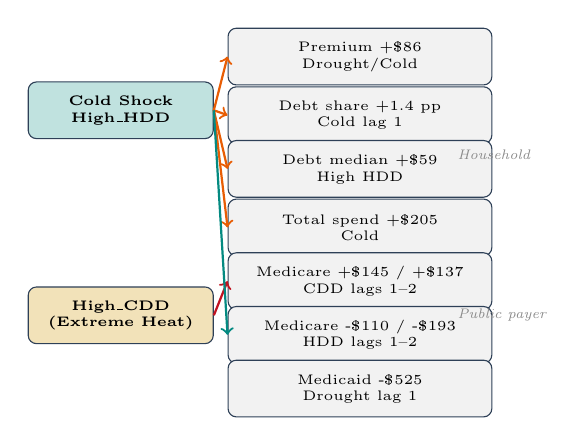
\begin{tikzpicture}[scale=0.62,
        box/.style={draw=DeepNavy, rounded corners=3pt, fill=LightGray,
                    minimum width=3.35cm, minimum height=0.72cm,
                    align=center, font=\tiny},
        cause/.style={draw=DeepNavy, rounded corners=3pt,
                    minimum width=2.35cm, minimum height=0.72cm,
                    align=center, font=\tiny\bfseries}]

        % Cause nodes
        \node[cause, fill=Teal!25]  (cold) at (0, 0)    {Cold Shock\\High\_HDD};
        \node[cause, fill=Gold!30]  (heat) at (0,-4.2)  {High\_CDD\\(Extreme Heat)};

        % Outcome nodes — household channel
        \node[box] (prem)  at (4.9, 1.1)  {Premium +\$86\\Drought/Cold};
        \node[box] (dshare) at (4.9,-0.1) {Debt share +1.4 pp\\Cold lag 1};
        \node[box] (dmed)  at (4.9,-1.2)  {Debt median +\$59\\High HDD};
        \node[box] (exp)   at (4.9,-2.4)  {Total spend +\$205\\Cold};

        % Outcome nodes — public payer channel
        \node[box] (mc1)   at (4.9,-3.5)  {Medicare +\$145 / +\$137\\CDD lags 1--2};
        \node[box] (mc2)   at (4.9,-4.6)  {Medicare -\$110 / -\$193\\HDD lags 1--2};
        \node[box] (mcd)   at (4.9,-5.7)  {Medicaid -\$525\\Drought lag 1};

        % Arrows
        \draw[->, WarmOrange, thick] (cold.east) -- (prem.west);
        \draw[->, WarmOrange, thick] (cold.east) -- (dshare.west);
        \draw[->, WarmOrange, thick] (cold.east) -- (dmed.west);
        \draw[->, WarmOrange, thick] (cold.east) -- (exp.west);
        \draw[->, DeepRed,    thick] (heat.east) -- (mc1.west);
        \draw[->, Teal,       thick] (cold.east) -- (mc2.west);

        % Channel labels
        \node[font=\tiny\itshape, text=WarmGray, anchor=west] at (6.7,-0.9) {Household};
        \node[font=\tiny\itshape, text=WarmGray, anchor=west] at (6.7,-4.2) {Public payer};
      \end{tikzpicture}
      \end{center}
    \end{column}
    \begin{column}{0.41\textwidth}
      \footnotesize
      \textbf{Cold channel:}
      \begin{itemize}\itemsep0.10em
        \item Premiums, debt, and total spending rise
        \item Medicare falls with lagged HDD exposure
      \end{itemize}
      \vspace{0.15em}
      \textbf{Heat channel (CDD):}
      \begin{itemize}\itemsep0.10em
        \item Medicare rises 1--2 years later
      \end{itemize}
      \vspace{0.15em}
      \textbf{Drought:}
      \begin{itemize}\itemsep0.10em
        \item Medicaid falls and premiums rise
      \end{itemize}
      \vspace{0.15em}
      \tealtext{\footnotesize Heat and cold affect public payers in\\opposite directions — novel finding.}
    \end{column}
  \end{columns}
\end{frame}

% ── Slide 3: State — Household / Individual Outcomes ─────────────────────────
\begin{frame}{State: Drought and Cold Raise Premiums and Debt}
  \framesubtitle{Household \& individual outcomes; $^{*}p{<}0.10$, $^{**}p{<}0.05$, $^{***}p{<}0.01$}
  \small
  \begin{columns}[T]
    \begin{column}{0.50\textwidth}
      \tealtext{\textbf{Employer Premium Contribution (\$/yr)}}\\[0.25em]
      \begin{tabular}{lrl}
        \toprule
        Predictor & Coef. & \\
        \midrule
        Extreme Drought ($h{=}0$)  & $+63.6$  & \emphcolor{**}  \\
        Severe Drought ($h{=}0$)   & $+86.4$  & \emphcolor{***} \\
        Severe Drought (lag 1)     & $+65.1$  & \emphcolor{**}  \\
        Pct PM$_{2.5}$ days        & $+20.8$  & \emphcolor{***} \\
        Pct PM$_{10}$ days         & $+22.7$  & \emphcolor{***} \\
        Pct Ozone days             & $+19.7$  & \emphcolor{***} \\
        \bottomrule
      \end{tabular}
      \vspace{0.4em}
      \graytext{\scriptsize Air quality pollutant days show consistent\\positive effects on employer premium costs.}
    \end{column}
    \begin{column}{0.46\textwidth}
      \tealtext{\textbf{Medical Debt Share (pp)}}\\[0.25em]
      \begin{tabular}{lrl}
        \toprule
        Predictor & Coef. & \\
        \midrule
        Cold Shock (lag 1) & $+0.0135$ & \emphcolor{**} \\
        \bottomrule
      \end{tabular}
      \vspace{0.5em}

      \tealtext{\textbf{Medical Debt Median (\$/yr)}}\\[0.25em]
      \begin{tabular}{lrl}
        \toprule
        Predictor & Coef. & \\
        \midrule
        High HDD ($h{=}0$)       & $+58.9$  & \emphcolor{**}  \\
        Severe Drought ($h{=}0$) & $-66.8$  & \emphcolor{***} \\
        Severe Drought (lag 1)   & $-37.5$  & \emphcolor{**}  \\
        Heat Shock ($h{=}0$)     & $+32.7$  & \emphcolor{*}   \\
        Heat Shock (lag 2)       & $+47.7$  & \emphcolor{**}  \\
        \bottomrule
      \end{tabular}
      \vspace{0.2em}
      \graytext{\scriptsize Cold raises debt prevalence; drought\\paradoxically reduces median severity.}
    \end{column}
  \end{columns}
\end{frame}

% ── Slide 4: State — Hospital & System Outcomes ───────────────────────────────
\begin{frame}{State: Cold Raises System Costs; Drought Cuts Public Payer Spending}
  \framesubtitle{Hospital \& system outcomes; two-way FE (State + Year)}
  \scriptsize
  \begin{columns}[T]
    \begin{column}{0.50\textwidth}
      \tealtext{\textbf{Total Per-Capita Health Expenditure (\$)}}\\[0.25em]
      \begin{tabular}{lrl}
        \toprule
        Predictor & Coef. & \\
        \midrule
        Cold Shock ($h{=}0$)   & $+205.3$ & \emphcolor{**} \\
        High HDD (lag 2)       & $+92.0$  & \emphcolor{*}  \\
        \bottomrule
      \end{tabular}
      \vspace{0.45em}

      \tealtext{\textbf{Medicaid per Enrollee (\$)}}\\[0.25em]
      \begin{tabular}{lrl}
        \toprule
        Predictor & Coef. & \\
        \midrule
        Extreme Drought ($h{=}0$) & $-566.2$ & \emphcolor{**}  \\
        Severe Drought ($h{=}0$)  & $-525.8$ & \emphcolor{**}  \\
        Severe Drought (lag 1)    & $-524.5$ & \emphcolor{***} \\
        Severe Drought (lag 2)    & $-288.4$ & \emphcolor{**}  \\
        \bottomrule
      \end{tabular}
      \vspace{0.2em}
      \graytext{\scriptsize Drought persistently reduces Medicaid\\spending across lags 0--2.}
    \end{column}
    \begin{column}{0.46\textwidth}
      \tealtext{\textbf{Medicare per Enrollee (\$)}}\\[0.25em]
      \begin{tabular}{lrl}
        \toprule
        Predictor & Coef. & \\
        \midrule
        Severe Drought (lag 1)   & $-144.3$ & \emphcolor{***} \\
        High CDD (lag 1)         & $+144.7$ & \emphcolor{**}  \\
        High CDD (lag 2)         & $+137.2$ & \emphcolor{***} \\
        High HDD (lag 1)         & $-110.1$ & \emphcolor{*}   \\
        High HDD (lag 2)         & $-192.7$ & \emphcolor{***} \\
        Unhealthy days & $+97.7$  & \emphcolor{**}  \\
        \bottomrule
      \end{tabular}
      \vspace{0.2em}
      \graytext{\scriptsize Heat (CDD) raises Medicare with lag;\\cold (HDD) reduces it — opposite channels.}
    \end{column}
  \end{columns}
\end{frame}

% ── State interpretation ──────────────────────────────────────────────────────
\begin{frame}[shrink=18]{State Results: Plain-English Interpretation}
  \framesubtitle{What do these coefficients mean for a real state?}
  \begin{columns}[T]
    \begin{column}{0.48\textwidth}
      \textbf{\tealtext{Cold shock (High HDD) raises premiums}}\\[0.2em]
      \footnotesize
      A year with extreme heating degree days raises the Benchmark Silver premium by \emphcolor{+\$86/month} for severe drought conditions or around +\$28--\$63 depending on drought severity. For a family of four, that is \emphcolor{+\$1,000--\$4,000 per year} in insurance costs during a bad cold year.\\[0.4em]
      \textbf{\tealtext{Drought suppresses Medicaid spending}}\\[0.2em]
      Extreme drought reduces Medicaid per-enrollee spending by \emphcolor{--\$525} in the same year and remains negative for two further years. This is \emph{not} good news: it likely reflects \emphcolor{forgone care} --- fewer doctor visits during economic stress, not lower medical need.
    \end{column}
    \begin{column}{0.48\textwidth}
      \textbf{\tealtext{Heat raises Medicare with delay}}\\[0.2em]
      \footnotesize
      Extreme CDD years raise Medicare per-enrollee spending by \emphcolor{+\$137--\$145} at lags 1--2. The elderly are most vulnerable to heat-related illness; their costs appear in the Medicare budget 1--2 years after the shock (hospitalisation, follow-up care).\\[0.4em]
      \textbf{\tealtext{Heat and cold push Medicare in opposite directions}}\\[0.2em]
      Cold (HDD) \emph{reduces} Medicare with lag ($-\$110$ to $-\$193$). The asymmetry suggests different mechanisms: cold stress triggers emergency use that is absorbed privately or via Medicaid, while heat stress generates Medicare-relevant chronic-disease exacerbation.\\[0.3em]
      \graytext{\scriptsize \textbf{Summary:} cold damages household and private insurance; drought damages the public safety net; heat shifts costs to Medicare.}
    \end{column}
  \end{columns}
\end{frame}

% ━━━━━━━━━━━━━━━━━━━━━━━━━━━━━━━━━━━━━━━━━━━━━━━━━━━━━━━━━━━━━━━━━━━━━━━━━━━
% SECTION B — COUNTY: HOUSEHOLD & INDIVIDUAL
% ━━━━━━━━━━━━━━━━━━━━━━━━━━━━━━━━━━━━━━━━━━━━━━━━━━━━━━━━━━━━━━━━━━━━━━━━━━━
\transitionslide{County Results: Household \& Individual}{Medical debt, premiums, income, employment\\Two-way FE: County + Year,\ \ N\(\approx\)23k--34k,\ \ cluster = State}

% ── Slide: County — Cold vs. Heat Channel Diagram ────────────────────────────
\begin{frame}{County-Level: Cold and Heat Channels Mirror the State Findings}
  \begin{columns}[T]
    \begin{column}{0.58\textwidth}
      \vspace{0.2em}
      \begin{center}
      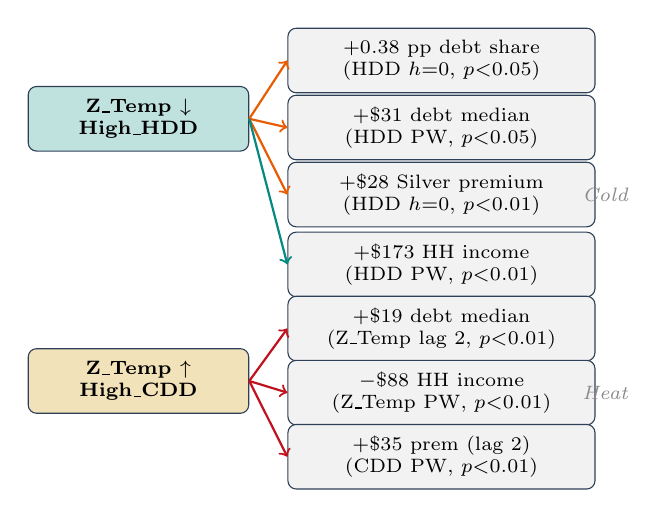
\begin{tikzpicture}[scale=0.74,
        box/.style={draw=DeepNavy, rounded corners=3pt, fill=LightGray,
                    minimum width=3.9cm, minimum height=0.82cm,
                    align=center, font=\scriptsize},
        cause/.style={draw=DeepNavy, rounded corners=3pt,
                    minimum width=2.8cm, minimum height=0.82cm,
                    align=center, font=\scriptsize\bfseries}]

        % Cause nodes
        \node[cause, fill=Teal!25]  (cold) at (0, 0)    {Z\_Temp $\downarrow$\\High\_HDD};
        \node[cause, fill=Gold!30]  (heat) at (0,-4.5)  {Z\_Temp $\uparrow$\\High\_CDD};

        % Household outcomes from cold
        \node[box] (dshare) at (5.2, 1.0)  {$+0.38$ pp debt share\\(HDD $h{=}0$, $p{<}0.05$)};
        \node[box] (dmed)   at (5.2,-0.15) {$+\$31$ debt median\\(HDD PW, $p{<}0.05$)};
        \node[box] (prem)   at (5.2,-1.3)  {$+\$28$ Silver premium\\(HDD $h{=}0$, $p{<}0.01$)};
        \node[box] (hinc)   at (5.2,-2.5)  {$+\$173$ HH income\\(HDD PW, $p{<}0.01$)};

        % Household outcomes from heat
        \node[box] (dmed2)  at (5.2,-3.6)  {$+\$19$ debt median\\(Z\_Temp lag 2, $p{<}0.01$)};
        \node[box] (hinc2)  at (5.2,-4.7)  {$-\$88$ HH income\\(Z\_Temp PW, $p{<}0.01$)};
        \node[box] (prem2)  at (5.2,-5.8)  {$+\$35$ prem (lag 2)\\(CDD PW, $p{<}0.01$)};

        % Arrows
        \draw[->, WarmOrange, thick] (cold.east) -- (dshare.west);
        \draw[->, WarmOrange, thick] (cold.east) -- (dmed.west);
        \draw[->, WarmOrange, thick] (cold.east) -- (prem.west);
        \draw[->, Teal,       thick] (cold.east) -- (hinc.west);
        \draw[->, DeepRed,    thick] (heat.east) -- (dmed2.west);
        \draw[->, DeepRed,    thick] (heat.east) -- (hinc2.west);
        \draw[->, DeepRed,    thick] (heat.east) -- (prem2.west);

        % Channel labels
        \node[font=\scriptsize\itshape, text=WarmGray, anchor=west] at (7.45,-1.3) {Cold};
        \node[font=\scriptsize\itshape, text=WarmGray, anchor=west] at (7.45,-4.7) {Heat};
      \end{tikzpicture}
      \end{center}
    \end{column}
    \begin{column}{0.38\textwidth}
      \scriptsize
      \textbf{Cold channel:}
      \begin{itemize}\itemsep0.05em
        \item Raises debt prevalence and severity
        \item Raises premiums on impact
        \item \tealtext{Raises} HH income (energy mix?)
      \end{itemize}
      \vspace{0.1em}
      \textbf{Heat channel:}
      \begin{itemize}\itemsep0.05em
        \item Raises debt median (lagged)
        \item \emphcolor{Reduces} HH income contemporaneously
        \item Raises premiums with 1--2 yr lag
      \end{itemize}
      \vspace{0.1em}
      \textbf{Cross-level:}
      \begin{itemize}\itemsep0.05em
        \item Cold $\to$ debt: both levels confirmed
        \item Heat $\to$ income: county only
        \item Premium channels align in direction
      \end{itemize}
    \end{column}
  \end{columns}
\end{frame}

% ── Slide 7: County — Medical Debt ───────────────────────────────────────────
\begin{frame}{County: Heat Raises Debt Severity; Cold Raises Debt Prevalence}
  \framesubtitle{Medical Debt Share (pp) and Median Debt (\$2023); UW = unweighted, PW = pop-weighted}
  \small
  \begin{columns}[T]
    \begin{column}{0.47\textwidth}
      \tealtext{\textbf{Z\_Temp (Relative Heat Shock)}}\\[0.3em]
      \begin{tabular}{lcc}
        \toprule
        & UW & PW \\
        \midrule
        \multicolumn{3}{l}{\textit{Debt Share (pp)}} \\
        $h{=}0$  & $-0.0025^{*}$  & $-0.0000$ \\
        Lag 2    & \emphcolor{$-0.0027^{**}$} & \emphcolor{$-0.0014^{*}$} \\[0.3em]
        \multicolumn{3}{l}{\textit{Debt Median (\$)}} \\
        $h{=}0$  & \emphcolor{$+14.9^{*}$}   & \emphcolor{$+18.5^{***}$} \\
        Lag 2    & \emphcolor{$+19.5^{**}$}  & \emphcolor{$+16.2^{***}$} \\
        \bottomrule
      \end{tabular}
      \vspace{0.35em}
      \graytext{\scriptsize Heat reduces prevalence but raises severity\\--- consistent composition effect:\\warm years shed marginal debtors while\\pushing the remaining cases deeper.}
    \end{column}
    \begin{column}{0.47\textwidth}
      \tealtext{\textbf{High\_HDD (Extreme Cold Burden)}}\\[0.3em]
      \begin{tabular}{lcc}
        \toprule
        & UW & PW \\
        \midrule
        \multicolumn{3}{l}{\textit{Debt Share (pp)}} \\
        $h{=}0$  & \emphcolor{$+0.0038^{**}$} & \emphcolor{$+0.0054^{**}$} \\
        Lag 2    & $+0.0031^{*}$  & $+0.0037^{*}$  \\[0.3em]
        \multicolumn{3}{l}{\textit{Debt Median (\$)}} \\
        $h{=}0$  & $+10.6$        & \emphcolor{$+31.2^{**}$}  \\
        \bottomrule
      \end{tabular}
      \vspace{0.35em}
      \textbf{Controls (all debt models):}\\[0.2em]
      \begin{tabular}{lc}
        Uninsured Rate & \emphcolor{$+^{***}$ (large)} \\
        HH Income      & \emphcolor{$-^{**}$} \\
      \end{tabular}
      \vspace{0.2em}\\
      \graytext{\scriptsize Cold raises both prevalence and severity\\--- no composition effect.}
    \end{column}
  \end{columns}
\end{frame}

% ── Slide 8: County — Premiums ────────────────────────────────────────────────
\begin{frame}{County: Cold Raises Premiums Now; Heat Raises Them Later}
  \framesubtitle{Benchmark Silver Premium (\$2023 real); county + year FE}
  \scriptsize
  \begin{columns}[T]
    \begin{column}{0.47\textwidth}
      \tealtext{\textbf{High\_HDD (Cold Burden)}}\\[0.25em]
      \begin{tabular}{lrrl}
        \toprule
        Lag & UW & PW & Cluster \\
        \midrule
        $h{=}0$ & \emphcolor{$+28.1^{***}$} & \emphcolor{$+21.9^{**}$}  & State \\
        $h{=}0$ & \emphcolor{$+28.1^{***}$} & \emphcolor{$+21.9^{***}$} & RA    \\
        Lag 1   & $-24.5^{*}$  & $-20.8$  & State \\
        \bottomrule
      \end{tabular}
      \vspace{0.4em}

      \tealtext{\textbf{High\_CDD (Heat Burden) — lagged}}\\[0.25em]
      \begin{tabular}{lrrl}
        \toprule
        Lag & UW & PW & Cluster \\
        \midrule
        Lag 1 & $+8.7$  & \emphcolor{$+31.4^{***}$} & RA \\
        Lag 2 & \emphcolor{$+21.6^{*}$} & \emphcolor{$+35.3^{***}$} & RA \\
        \bottomrule
      \end{tabular}
    \end{column}
    \begin{column}{0.47\textwidth}
      \tealtext{\textbf{Z\_Temp (Relative Temp)}}\\[0.25em]
      \begin{tabular}{lrrl}
        \toprule
        Lag & UW & PW & Cluster \\
        \midrule
        $h{=}0$ & \emphcolor{$-10.9^{**}$} & $+2.7$  & RA \\
        Lag 1   & $+3.8$  & \emphcolor{$+5.4^{**}$}  & RA \\
        Lag 2   & $+1.0$  & \emphcolor{$+4.2^{**}$}  & RA \\
        \bottomrule
      \end{tabular}
      \vspace{0.25em}
      \begin{itemize}\itemsep0.14em
        \item \emphcolor{Cold (HDD)} raises premiums on impact in both state- and RA-clustered specs
        \item \emphcolor{Heat} lowers premiums now, then raises them 1--2 years later
        \item RA clustering tightens CIs; drought lag 1 is borderline at $+\$3.9$ ($p{=}0.05$)
      \end{itemize}
    \end{column}
  \end{columns}
\end{frame}

% ── Slide 9: County — Income & Employment ────────────────────────────────────
\begin{frame}[shrink=12]{County: Heat Depresses Income; Drought Hits PCPI}
  \framesubtitle{Median HH income and per-capita personal income (\$2023)}
  \small
  \begin{columns}[T]
    \begin{column}{0.48\textwidth}
      \tealtext{\textbf{Median HH Income (\$2023)}}\\[0.25em]
      \begin{tabular}{lcc}
        \toprule
        Predictor & UW & PW \\
        \midrule
        Z\_Temp ($h{=}0$)   & \emphcolor{$-71^{**}$}  & \emphcolor{$-88^{***}$} \\
        Z\_Temp (lag 1)     & $-36$  & \emphcolor{$-64^{***}$} \\
        Z\_Temp (lag 2)     & \emphcolor{$-71^{**}$}  & \emphcolor{$-60^{**}$}  \\
        High\_CDD ($h{=}0$) & \emphcolor{$-247^{**}$} & $-3$   \\
        High\_HDD ($h{=}0$) & $+161^{**}$ & \emphcolor{$+173^{***}$} \\
        \bottomrule
      \end{tabular}
      \vspace{0.25em}
      \graytext{\scriptsize Relative heat most consistently lowers household income in the population-weighted specifications.}

      \tealtext{\textbf{Per-Capita Personal Income (\$)}}\\[0.25em]
      \begin{tabular}{lcc}
        \toprule
        Predictor & UW & PW \\
        \midrule
        PDSI lag 2             & $-8.5$  & \emphcolor{$-113^{**}$} \\
        High\_CDD lag 1        & \emphcolor{$+480^{**}$} & $-116$ \\
        RA-level: PDSI ($h{=}0$) & \multicolumn{2}{c}{\emphcolor{$-206^{***}$}} \\
        \bottomrule
      \end{tabular}
    \end{column}
    \begin{column}{0.46\textwidth}
      \tealtext{\textbf{Income Summary}}\\[0.25em]
      \begin{itemize}\itemsep0.16em
        \item \emphcolor{Heat} lowers HH income across lags in pop-weighted models
        \item \emphcolor{Cold} raises HH income on impact, likely reflecting seasonal or energy-income composition
        \item \emphcolor{Drought} is strongest in PCPI: RA spec gives $-\$206^{***}$
      \end{itemize}
      \vspace{0.25em}
      \tealtext{\textbf{Civilian Employment (persons)}}\\[0.25em]
      \begin{tabular}{lcc}
        \toprule
        Predictor & UW & PW \\
        \midrule
        Z\_Temp lag 2       & \emphcolor{$+788^{**}$} & $+3216$ \\
        High\_HDD ($h{=}0$) & \emphcolor{$-468^{**}$} & $+2587$ \\
        High\_HDD lag 2     & \emphcolor{$-678^{**}$} & $+3988$ \\
        Z\_Precip ($h{=}0$) & $+46$   & \emphcolor{$-5742^{***}$} \\
        Z\_Precip (lag 1)   & $-88$   & \emphcolor{$-3803^{***}$} \\
        \bottomrule
      \end{tabular}
      \vspace{0.25em}
      \begin{itemize}\itemsep0.16em
        \item \emphcolor{Cold} suppresses employment in unweighted county models
        \item \emphcolor{Precipitation shocks} are strongly negative in population-weighted specifications
        \item Employment results are more weighting-sensitive than the income results
        \item RA-level: drought reduces PCPI $-\$206^{***}$ — strongest signal in the income block
      \end{itemize}
    \end{column}
  \end{columns}
\end{frame}

% ── Slide 10: County — Cold vs. Heat Channel Diagram ─────────────────────────
\begin{frame}{County-Level: Cold and Heat Channels Mirror the State Findings}
  \begin{columns}[T]
    \begin{column}{0.58\textwidth}
      \vspace{0.2em}
      \begin{center}
      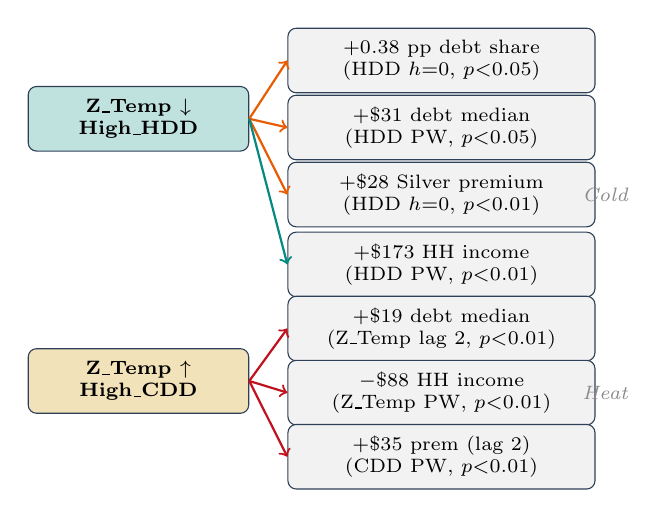
\begin{tikzpicture}[scale=0.74,
        box/.style={draw=DeepNavy, rounded corners=3pt, fill=LightGray,
                    minimum width=3.9cm, minimum height=0.82cm,
                    align=center, font=\scriptsize},
        cause/.style={draw=DeepNavy, rounded corners=3pt,
                    minimum width=2.8cm, minimum height=0.82cm,
                    align=center, font=\scriptsize\bfseries}]

        % Cause nodes
        \node[cause, fill=Teal!25]  (cold) at (0, 0)    {Z\_Temp $\downarrow$\\High\_HDD};
        \node[cause, fill=Gold!30]  (heat) at (0,-4.5)  {Z\_Temp $\uparrow$\\High\_CDD};

        % Household outcomes from cold
        \node[box] (dshare) at (5.2, 1.0)  {$+0.38$ pp debt share\\(HDD $h{=}0$, $p{<}0.05$)};
        \node[box] (dmed)   at (5.2,-0.15) {$+\$31$ debt median\\(HDD PW, $p{<}0.05$)};
        \node[box] (prem)   at (5.2,-1.3)  {$+\$28$ Silver premium\\(HDD $h{=}0$, $p{<}0.01$)};
        \node[box] (hinc)   at (5.2,-2.5)  {$+\$173$ HH income\\(HDD PW, $p{<}0.01$)};

        % Household outcomes from heat
        \node[box] (dmed2)  at (5.2,-3.6)  {$+\$19$ debt median\\(Z\_Temp lag 2, $p{<}0.01$)};
        \node[box] (hinc2)  at (5.2,-4.7)  {$-\$88$ HH income\\(Z\_Temp PW, $p{<}0.01$)};
        \node[box] (prem2)  at (5.2,-5.8)  {$+\$35$ prem (lag 2)\\(CDD PW, $p{<}0.01$)};

        % Arrows
        \draw[->, WarmOrange, thick] (cold.east) -- (dshare.west);
        \draw[->, WarmOrange, thick] (cold.east) -- (dmed.west);
        \draw[->, WarmOrange, thick] (cold.east) -- (prem.west);
        \draw[->, Teal,       thick] (cold.east) -- (hinc.west);
        \draw[->, DeepRed,    thick] (heat.east) -- (dmed2.west);
        \draw[->, DeepRed,    thick] (heat.east) -- (hinc2.west);
        \draw[->, DeepRed,    thick] (heat.east) -- (prem2.west);

        % Channel labels
        \node[font=\scriptsize\itshape, text=WarmGray, anchor=west] at (7.45,-1.3) {Cold};
        \node[font=\scriptsize\itshape, text=WarmGray, anchor=west] at (7.45,-4.7) {Heat};
      \end{tikzpicture}
      \end{center}
    \end{column}
    \begin{column}{0.38\textwidth}
      \scriptsize
      \textbf{Cold channel:}
      \begin{itemize}\itemsep0.05em
        \item Raises debt prevalence and severity
        \item Raises premiums on impact
        \item \tealtext{Raises} HH income (energy mix?)
      \end{itemize}
      \vspace{0.1em}
      \textbf{Heat channel:}
      \begin{itemize}\itemsep0.05em
        \item Raises debt median (lagged)
        \item \emphcolor{Reduces} HH income contemporaneously
        \item Raises premiums with 1--2 yr lag
      \end{itemize}
      \vspace{0.1em}
      \textbf{Cross-level:}
      \begin{itemize}\itemsep0.05em
        \item Cold $\to$ debt: both levels confirmed
        \item Heat $\to$ income: county only
        \item Premium channels align in direction
      \end{itemize}
    \end{column}
  \end{columns}
\end{frame}

% ── County vs State comparison ────────────────────────────────────────────────
\begin{frame}[shrink=18]{County vs.\ State: Why More Granularity Changes What We Find}
  \framesubtitle{County FE absorbs within-state heterogeneity invisible to state models}
  \begin{columns}[T]
    \begin{column}{0.48\textwidth}
      \textbf{\tealtext{What county models add}}\\[0.2em]
      \footnotesize
      \begin{itemize}\itemsep0.16em
        \item State models average over 3,000+ counties --- rural and urban, coastal and inland, insured and uninsured. County models let each county serve as its own control.
        \item \emphcolor{Heat $\to$ household income loss}: not visible in state models, emerges clearly in county models ($-\$88^{***}$ per capita). Likely masked by state-level averaging with opposite-direction rural/urban effects.
        \item \emphcolor{Cold $\to$ hospital bad debt}: county-level variation ($+\$5/capita$) is not detectable in the $N=650$ state panel.
        \item \emphcolor{Rating-area structure}: premiums are set at the rating-area level. County models with rating-area clustering are the correct specification.
      \end{itemize}
    \end{column}
    \begin{column}{0.48\textwidth}
      \textbf{\tealtext{Where state and county agree}}\\[0.2em]
      \footnotesize
      \begin{itemize}\itemsep0.16em
        \item Cold $\to$ debt and premiums: confirmed at both levels
        \item Drought $\to$ public payer suppression: both levels significant
        \item Heat $\to$ delayed premium increases: both levels
        \item Air quality $\to$ employer premiums: state level (state AQI); county level uses Max AQI shock indicator
      \end{itemize}
      \vspace{0.3em}
      \textbf{\tealtext{Sample size and power}}\\[0.2em]
      \begin{itemize}\itemsep0.12em
        \item State: $N \approx 650$; County: $N \approx 23{,}000$--$34{,}000$
        \item County panel has $\sim$50$\times$ more observations
        \item Allows detection of effects too small to identify at state level
      \end{itemize}
    \end{column}
  \end{columns}
\end{frame}

% ━━━━━━━━━━━━━━━━━━━━━━━━━━━━━━━━━━━━━━━━━━━━━━━━━━━━━━━━━━━━━━━━━━━━━━━━━━━
% SECTION C — COUNTY: HOSPITAL
% ━━━━━━━━━━━━━━━━━━━━━━━━━━━━━━━━━━━━━━━━━━━━━━━━━━━━━━━━━━━━━━━━━━━━━━━━━━━
\transitionslide{County Results: Hospital Sector}{Hospital bad debt per capita\\Two-way FE: County + Year,\ \ N\(\approx\)27k,\ \ cluster = State}

% ── Slide 12: County — Hospital Bad Debt ─────────────────────────────────────
\begin{frame}{County: Cold Raises Hospital Bad Debt; Heat Lag Reduces It}
  \framesubtitle{Hospital Bad Debt per Capita (\$); within-R$^2 = 0.006$--$0.019$}
  \scriptsize
  \begin{columns}[T]
    \begin{column}{0.47\textwidth}
      \tealtext{\textbf{Key Coefficient Estimates}}\\[0.3em]
      \begin{tabular}{lcc}
        \toprule
        Predictor & UW & PW \\
        \midrule
        Z\_Temp lag 2       & \emphcolor{$-2.41^{***}$} & \emphcolor{$-2.08^{***}$} \\
        Z\_Temp ($h{=}0$)   & $-1.25$  & \emphcolor{$-1.08^{**}$} \\
        High\_HDD ($h{=}0$) & \emphcolor{$+5.33^{***}$} & \emphcolor{$+4.23^{**}$} \\
        PDSI lag 1          & $+0.57^{*}$ & $+0.50^{*}$ \\
        PDSI lag 2          & $+0.01$ & \emphcolor{$+0.50^{*}$} \\
        Uninsured Rate      & \emphcolor{$+151^{***}$}  & $+142$ \\
        \bottomrule
      \end{tabular}
      \vspace{0.35em}
      \graytext{\scriptsize RA-level robustness (pop-wtd):\\PDSI lag 2: $+0.76^{***}$\quad Z\_Temp lag 2: $-2.26^{***}$}
    \end{column}
    \begin{column}{0.47\textwidth}
      \begin{itemize}\itemsep0.18em
        \item \emphcolor{Cold (HDD) raises bad debt on impact} by \$4--5 per capita — consistent with emergency utilisation, deferred billing, and coverage gaps during cold events
        \item \emphcolor{Heat lag reduces bad debt} (2-yr lag, $p{<}0.001$) — possible reduction in elective utilisation during hot years or survivor selection
        \item \emphcolor{PDSI (drought)} adds a smaller lagged increase, confirmed in RA robustness
        \item \emphcolor{Uninsured Rate} is the dominant control ($+151^{***}$ unweighted) — structural coverage gap drives hospital write-offs
      \end{itemize}
      \vspace{0.2em}
      \graytext{\scriptsize About 23\% of county-years lack hospital reports; one negative outlier is winsorized.}
    \end{column}
  \end{columns}
\end{frame}

% ━━━━━━━━━━━━━━━━━━━━━━━━━━━━━━━━━━━━━━━━━━━━━━━━━━━━━━━━━━━━━━━━━━━━━━━━━━━
% SECTION D — WEATHER SWING ANALYSIS
% ━━━━━━━━━━━━━━━━━━━━━━━━━━━━━━━━━━━━━━━━━━━━━━━━━━━━━━━━━━━━━━━━━━━━━━━━━━━
\transitionslide{Weather Swing Analysis}{A new source of variation: year-over-year climate volatility\\County + Year FE,\ \ N\(\approx\)23k--34k,\ \ cluster = State}

% ── Slide D1: Delta Methodology ──────────────────────────────────────────────
\begin{frame}{New Analysis: Exploiting Year-to-Year Weather Swings}
  \framesubtitle{County-level only; $N{\approx}650$ state-years insufficient for first-difference identification}
  \begin{columns}[T]
    \begin{column}{0.48\textwidth}
      \textbf{\tealtext{Motivation}}\\[0.15em]
      \footnotesize
      \begin{itemize}\itemsep0.12em
        \item Prior specs identify counties in persistent shock states vs.\ not
        \item New margin: do counties that \emphcolor{swing sharply} year-to-year bear extra health costs, regardless of average climate?
        \item Is it \emphcolor{volatility}, not just level, that damages health finance?
      \end{itemize}
      \vspace{0.2em}
      \textbf{\tealtext{Robustness Specs}}\\[0.1em]
      \footnotesize
      \begin{itemize}\itemsep0.10em
        \item \emphcolor{Asymmetric:} $\Delta^{+} = \max(\Delta X, 0)$ vs.\ $\Delta^{-} = \min(\Delta X, 0)$
        \item \emphcolor{Binary transitions:} Onset / Exit / Persist indicators
      \end{itemize}
    \end{column}
    \begin{column}{0.48\textwidth}
      \textbf{\tealtext{Primary Specification}}\\[0.15em]
      \footnotesize
      \[
        Y_{it} = \alpha_i + \gamma_t + \beta_1 \underbrace{\Delta X_{it}}_{\text{swing}} + \beta_2 \underbrace{X_{i,t-1}}_{\text{lagged level}} + \mathbf{X}_{it}'\delta + \varepsilon_{it}
      \]
      \begin{itemize}\itemsep0.12em
        \item $\Delta X_{it} = X_{it} - X_{i,t-1}$ for all continuous exposures:\\
              \texttt{Z\_Temp, Z\_Precip, CDD, HDD, PDSI, Median\_AQI, Max\_AQI}
        \item $\beta_2$ controls for prior-year level --- isolates pure swing effect
        \item LP extension: $Y_{i,t+h}$ at $h = 0, 1, 2, 3$
        \item County + year FE; state-clustered SEs
      \end{itemize}
    \end{column}
  \end{columns}
\end{frame}

% ── Slide D1b: Why first differences? ────────────────────────────────────────
\begin{frame}[shrink=18]{First Differences as a Design Choice: What Exactly Are We Estimating?}
  \framesubtitle{The difference between level effects and swing effects}
  \begin{columns}[T]
    \begin{column}{0.50\textwidth}
      \textbf{\tealtext{Level effects (Phase 2)}}\\[0.2em]
      \footnotesize
      \begin{itemize}\itemsep0.14em
        \item Asks: do counties that experience \emphcolor{more extreme shocks} in a given year have higher health costs that year (or 1--2 years later)?
        \item Identifies the effect of shock \emph{occurrence} vs.\ no shock
        \item Cannot detect whether \emphcolor{rapid change} in climate exposure independently matters
      \end{itemize}
      \vspace{0.3em}
      \textbf{\tealtext{Swing effects (Phase 3)}}\\[0.2em]
      \begin{itemize}\itemsep0.14em
        \item Asks: does a county that shifts sharply \emphcolor{from one year to the next} bear extra costs, \emph{controlling for} where it was last year?
        \item Identifies the marginal effect of \emphcolor{volatility}
        \item Relevant for adaptation: a system that adapts to a persistent new climate level may still be damaged by rapid oscillation
      \end{itemize}
    \end{column}
    \begin{column}{0.46\textwidth}
      \textbf{\tealtext{A climate science analogy}}\\[0.2em]
      \footnotesize
      \begin{block}{}
        \scriptsize
        Compare two counties, both experiencing an ``extreme heat'' year (High CDD = 1). County A has had extreme heat for five consecutive years. County B is experiencing it for the first time after a run of mild summers. \emphcolor{Phase 2 gives both the same treatment indicator}. Phase 3 asks whether the \emph{shock of the transition} carries its own financial cost --- for B, $\Delta$CDD is large; for A, it is near zero.
      \end{block}
      \vspace{0.3em}
      \begin{itemize}\itemsep0.14em
        \item \emphcolor{Key insight from our data}: AQI level effects are consistently insignificant; AQI \emph{swings} are significant at all four LP horizons
        \item This suggests health systems have partially adapted to local chronic pollution but are \emphcolor{not adapted to sudden AQI shifts}
      \end{itemize}
    \end{column}
  \end{columns}
\end{frame}

% ── Slide D2: Delta Core Results ─────────────────────────────────────────────
\begin{frame}[shrink=5]{Weather Swings Affect Premiums, Debt, and Hospital Costs}
  \framesubtitle{Primary $\Delta$FE spec (h=0, unweighted); $^{*}p{<}0.10$,\ $^{**}p{<}0.05$,\ $^{***}p{<}0.01$}
  \small
  \begin{columns}[T]
    \begin{column}{0.47\textwidth}
      \tealtext{\textbf{$\Delta$HDD $\to$ Silver Premium}}\\[0.2em]
      \scriptsize
      \begin{tabular}{lcc}
        \toprule
        Spec & Estimate & $p$ \\
        \midrule
        $\Delta$HDD ($h{=}0$)   & \emphcolor{$+0.033^{***}$} & 0.0004 \\
        HDD Onset (binary)      & \emphcolor{$+49.46^{**}$}  & 0.0033 \\
        HDD\_Pos (asymm.)       & $+0.065^{*}$ & 0.028 \\
        \bottomrule
      \end{tabular}
      \vspace{0.25em}
      \graytext{\scriptsize Cold swing raises premiums on impact;\\onset of first extreme-cold year\\adds $\sim\$49$ to Silver benchmark.}

      \vspace{0.4em}
      \tealtext{\textbf{$\Delta$Z\_Temp $\to$ Medical Debt Median}}\\[0.2em]
      \begin{tabular}{lcc}
        \toprule
        Horizon & Estimate (\$) & $p$ \\
        \midrule
        $h{=}0$ & \emphcolor{$+13.2^{*}$}   & 0.014 \\
        $h{=}2$ & \emphcolor{$+19.4^{*}$}   & 0.033 \\
        $h{=}3$ & \emphcolor{$+29.7^{***}$} & 0.0001 \\
        \bottomrule
      \end{tabular}
      \vspace{0.2em}
      \graytext{\scriptsize Warming swing raises median debt\\with a growing 3-year lag.}
    \end{column}
    \begin{column}{0.47\textwidth}
      \tealtext{\textbf{$\Delta$Max\_AQI $\to$ Hospital Bad Debt (per capita)}}\\[0.2em]
      \scriptsize
      \begin{tabular}{lcc}
        \toprule
        Horizon & Estimate (\$) & $p$ \\
        \midrule
        $h{=}0$ & \emphcolor{$+0.0050^{**}$}  & 0.0014 \\
        $h{=}1$ & \emphcolor{$+0.0082^{***}$} & $<$0.001 \\
        $h{=}2$ & $+0.0080^{*}$               & 0.015 \\
        $h{=}3$ & \emphcolor{$+0.0157^{***}$} & $<$0.001 \\
        \bottomrule
      \end{tabular}
      \vspace{0.25em}
      \graytext{\scriptsize AQI swing effect on bad debt \emphcolor{grows} across\\all four horizons --- a persistent ratchet.\\Level effect was not significant in Phase 2.}

      \vspace{0.4em}
      \tealtext{\textbf{$\Delta$Z\_Precip / $\Delta$PDSI $\to$ PCPI}}\\[0.2em]
      \begin{tabular}{lcc}
        \toprule
        Exposure & $h{=}1$ est.\ & $p$ \\
        \midrule
        $\Delta$Z\_Precip & \emphcolor{$-274^{***}$} & 0.0006 \\
        $\Delta$PDSI      & \emphcolor{$-226^{***}$} & 0.0001 \\
        \bottomrule
      \end{tabular}
      \vspace{0.2em}
      \graytext{\scriptsize Precipitation and drought swings\\suppress per-capita income for 1--3 yrs.}
    \end{column}
  \end{columns}
\end{frame}

% ── Slide D3: Visual — LP dynamic profiles ───────────────────────────────────
\begin{frame}{Swing Effects Grow Over Time: Two Key LP Profiles}
  \framesubtitle{Local projection estimates at $h = 0,1,2,3$; county + year FE; state-clustered SEs; unweighted}
  \vspace{-0.2em}
  \begin{columns}[T]
    \begin{column}{0.48\textwidth}
      \begin{center}
        \textbf{\tealtext{\small $\Delta$Max\_AQI $\to$ Hospital Bad Debt (\$/capita)}}\\[0.1em]
        \includegraphics[width=\textwidth, height=0.46\textheight, keepaspectratio]%
          {../Analysis/plots/delta/lp_delta_Max_AQI_Hosp_BadDebt_PerCapita.png}
      \end{center}
      \vspace{-0.3em}
      \graytext{\scriptsize Effect grows at every horizon --- AQI bad-debt ratchet. Level effect was not significant in Phase 2.}
    \end{column}
    \begin{column}{0.48\textwidth}
      \begin{center}
        \textbf{\tealtext{\small $\Delta$Z\_Temp $\to$ Median Medical Debt (\$2023)}}\\[0.1em]
        \includegraphics[width=\textwidth, height=0.46\textheight, keepaspectratio]%
          {../Analysis/plots/delta/lp_delta_Z_Temp_Medical_Debt_Median_2023.png}
      \end{center}
      \vspace{-0.3em}
      \graytext{\scriptsize Warming swing accumulates into medical debt; $+\$30$ at $h{=}3$ ($p{<}0.001$).}
    \end{column}
  \end{columns}
\end{frame}

% ── Slide D4: Asymmetry & New vs. Prior Findings ─────────────────────────────
\begin{frame}{Asymmetry and Ratchets: Not All Swings Are Reversible}
  \framesubtitle{Asymmetric spec ($\Delta^{+}$ vs.\ $\Delta^{-}$) and onset/exit indicators}
  \begin{columns}[T]
    \begin{column}{0.47\textwidth}
      \textbf{\tealtext{Asymmetric Findings}}\\[0.15em]
      \footnotesize
      \begin{itemize}\itemsep0.13em
        \item \emphcolor{AQI ratchet:} improving air quality still raises bad debt ($\Delta^{-}$, $+0.010^{***}$) --- costs do not unwind when pollution falls
        \item \emphcolor{Drought worsening:} $\Delta^{-}$PDSI drives PCPI loss ($-207^{***}$); recovery asymmetrically weaker
        \item \emphcolor{CDD income:} symmetric --- cooling-sector PCPI moves with swings in both directions ($\pm 3.3$, $p{<}0.001$)
        \item \emphcolor{Drought exit} \emph{does} reduce medical debt ($-\$54^{*}$)
      \end{itemize}
    \end{column}
    \begin{column}{0.47\textwidth}
      \textbf{\tealtext{What the Delta Analysis Adds}}\\[0.15em]
      \footnotesize
      \renewcommand{\arraystretch}{1.25}
      \begin{tabular}{@{}>{\raggedright\arraybackslash}p{0.52\linewidth}>{\raggedright\arraybackslash}p{0.40\linewidth}@{}}
        \toprule
        Relationship & Finding \\
        \midrule
        AQI $\to$ hosp.\ bad debt & \emphcolor{New:} swing sig.; level not \\
        HDD $\to$ premiums & Confirms; adds onset pricing \\
        Drought $\to$ income & Confirms; worsening-only \\
        Temp swing $\to$ med.\ debt & New: 3-yr growing \\
        Precip swing $\to$ PCPI & New: 3-yr suppression \\
        \bottomrule
      \end{tabular}
      \vspace{0.2em}
      \graytext{\scriptsize \textbf{Key insight:} weather volatility carries independent health-finance costs beyond level effects.}
    \end{column}
  \end{columns}
\end{frame}

% ━━━━━━━━━━━━━━━━━━━━━━━━━━━━━━━━━━━━━━━━━━━━━━━━━━━━━━━━━━━━━━━━━━━━━━━━━━━
% SECTION E — SYNTHESIS
% ━━━━━━━━━━━━━━━━━━━━━━━━━━━━━━━━━━━━━━━━━━━━━━━━━━━━━━━━━━━━━━━━━━━━━━━━━━━
\transitionslide{Cross-Level Synthesis}{What do state, county, and swing analyses agree on?}

% ── Slide 14: Synthesis table ─────────────────────────────────────────────────
\begin{frame}{State and County Pipelines Tell a Consistent Story}
  \framesubtitle{Key findings replicated across both levels of analysis}
  \begin{center}
  \small
  \renewcommand{\arraystretch}{1.5}
  \begin{tabular}{lcc}
    \rowcolor{DeepNavy}
    \textcolor{white}{\textbf{Finding}} &
    \textcolor{white}{\textbf{State}} &
    \textcolor{white}{\textbf{County}} \\
    \rowcolor{Teal!10}
    Cold / HDD $\to$ medical debt (prevalence \& severity) &
    \tealtext{\textbf{\checkmark}} & \tealtext{\textbf{\checkmark}} \\
    Cold / HDD $\to$ higher premiums &
    \tealtext{\textbf{\checkmark}} \graytext{\scriptsize(via drought)} & \tealtext{\textbf{\checkmark}} \graytext{\scriptsize($p{<}0.01$)} \\
    \rowcolor{Teal!10}
    Cold / HDD $\to$ hospital bad debt $\uparrow$ &
    \graytext{---} & \tealtext{\textbf{\checkmark}} \graytext{\scriptsize($p{<}0.01$)} \\
    Drought $\to$ reduced Medicaid / PCPI &
    \tealtext{\textbf{\checkmark}} \graytext{\scriptsize($p{<}0.01$)} & \tealtext{\textbf{\checkmark}} \graytext{\scriptsize(PDSI)} \\
    \rowcolor{Teal!10}
    Heat $\to$ household income loss &
    \graytext{---} & \tealtext{\textbf{\checkmark}} \graytext{\scriptsize(Z\_Temp***)} \\
    Heat lag $\to$ Medicare / premiums $\uparrow$ &
    \tealtext{\textbf{\checkmark}} \graytext{\scriptsize(CDD***)} & \tealtext{\textbf{\checkmark}} \graytext{\scriptsize(CDD***)} \\
    \rowcolor{Teal!10}
    Heat lag $\to$ hospital bad debt $\downarrow$ &
    \graytext{---} & \tealtext{\textbf{\checkmark}} \graytext{\scriptsize($p{<}0.001$)} \\
    Poor air quality $\to$ higher premiums &
    \tealtext{\textbf{\checkmark}} \graytext{\scriptsize(PM$_{2.5}$/O$_3$***)} & \graytext{\scriptsize not modeled} \\
  \end{tabular}
  \end{center}
\end{frame}

% ── Caveats slide ─────────────────────────────────────────────────────────────
\begin{frame}[shrink=18]{Caveats and Limitations}
  \framesubtitle{What we can and cannot claim from this design}
  \begin{columns}[T]
    \begin{column}{0.48\textwidth}
      \textbf{\tealtext{What two-way FE cannot rule out}}\\[0.2em]
      \footnotesize
      \begin{itemize}\itemsep0.16em
        \item \emphcolor{Time-varying confounders}: a county-specific policy change (e.g.\ Medicaid expansion timing) that correlates with climate variation would contaminate the estimate. We control for observed time-varying covariates but cannot include everything.
        \item \emphcolor{Reverse causality}: unlikely here (climate is exogenous), but migration responses to climate shocks could affect measured outcomes.
        \item \emphcolor{Data quality}: hospital bad debt is self-reported; $\sim$23\% of county-years are missing. Medical debt from credit bureaus is a snapshot, not a flow.
      \end{itemize}
    \end{column}
    \begin{column}{0.48\textwidth}
      \textbf{\tealtext{Scope of claims}}\\[0.2em]
      \footnotesize
      \begin{itemize}\itemsep0.16em
        \item Results are \emphcolor{reduced-form associations} under two-way FE identification --- not causal in the IV sense
        \item \emphcolor{Short-run effects} only: the panel is 2011--2023. Long-run adaptation responses (e.g.\ insurer exit, hospital closure) are not captured
        \item \emphcolor{Weather swing analysis} captures short-run responsiveness to volatility; coefficients do not generalise to slow climate trends
        \item The medical debt reporting-rule exclusion (CO 2023) is conservative; it reduces rather than inflates the debt findings
      \end{itemize}
      \vspace{0.2em}
      \graytext{\scriptsize \textbf{Bottom line:} results are robust across multiple specifications, weighting approaches, and levels of analysis --- but should be interpreted as evidence of association, not a controlled experiment.}
    \end{column}
  \end{columns}
\end{frame}

% ── Policy implications ───────────────────────────────────────────────────────
\transitionslide{Policy Implications}{What should adaptation planners, insurers, and health systems take from this?}

\begin{frame}{Policy Implications: Climate Adaptation Must Include Health Finance}
  \framesubtitle{Three actionable implications for adaptation policy, insurer regulation, and health system design}
  \begin{columns}[T]
    \begin{column}{0.31\textwidth}
      \begin{alertblock}{Adaptation policy}
        \footnotesize
        \textbf{Current gap:} most adaptation frameworks target mortality and infrastructure.\\[0.4em]
        \textbf{Finding:} cold, drought, and AQI shocks increase medical debt and reduce income for 1--3 years after the event.\\[0.4em]
        \textbf{Implication:} \emphcolor{climate resilience funds} should include a health-finance window --- covering the period when households are financially recovering from a shock, not only emergency response.
      \end{alertblock}
    \end{column}
    \begin{column}{0.31\textwidth}
      \begin{exampleblock}{Insurance regulation}
        \footnotesize
        \textbf{Finding:} insurers raise ACA premiums in extreme cold years ($+\$28$--\$86) and after extreme heat ($+\$21$--\$35 at 1--2 yr lag). The swing analysis shows a cold \emph{onset} adds $\sim$\$49 instantly.\\[0.4em]
        \textbf{Implication:} regulators should \emphcolor{monitor climate-driven premium volatility} as a component of rate review. Counties transitioning into new climate regimes face a double burden: worsening shocks and rising insurance costs.
      \end{exampleblock}
    \end{column}
    \begin{column}{0.31\textwidth}
      \begin{block}{Hospital systems}
        \footnotesize
        \textbf{Finding:} hospital bad debt rises $+\$4$--\$5/capita in cold years and continues to grow after AQI swings for three years.\\[0.4em]
        \textbf{Finding:} drought worsening triggers income losses and employment falls simultaneously.\\[0.4em]
        \textbf{Implication:} \emphcolor{climate stress-testing} for hospital finances should use local climate volatility indices, not just long-run averages. Systems in high-volatility corridors need expanded charity-care reserves.
      \end{block}
    \end{column}
  \end{columns}
  \vspace{0.3em}
  \graytext{\scriptsize \textbf{Key message for climate scientists:} the downstream health-finance burden is measurable, large relative to program budgets, and exhibits hysteresis --- it does not recover automatically when weather improves.}
\end{frame}

% ── Slide 16: Next Steps ──────────────────────────────────────────────────────
\begin{frame}{Next Steps}
  \framesubtitle{Planned extensions to the empirical framework}
  \begin{columns}[T]
    \begin{column}{0.47\textwidth}
      \textbf{\tealtext{Empirical Extensions}}\\[-0.1em]
      \footnotesize
      \begin{itemize}\itemsep0.18em
        \item \emphcolor{Heterogeneity:} rural vs.\ urban and high- vs.\ low-AQI subsamples for both level and swing analyses
        \item \emphcolor{Mechanisms:} separate respiratory-illness from energy-poverty channels for cold shocks
        \item \emphcolor{County unemployment:} replace the ACS proxy with BLS LAUS series
        \item \emphcolor{Policy counterfactuals:} ACA Medicaid expansion $\times$ climate shocks
      \end{itemize}
    \end{column}
    \begin{column}{0.47\textwidth}
      \textbf{\tealtext{Writing and Defence}}\\[-0.1em]
      \footnotesize
      \begin{itemize}\itemsep0.18em
        \item \emphcolor{Chapter draft:} unify state, county, and swing narratives into a single empirical chapter
        \item \emphcolor{Swing robustness:} population-weighted LP profiles for delta results; cumulative IRF plots
        \item \emphcolor{Thesis write-up:} convert synthesis tables into publication-ready regression tables
      \end{itemize}
    \end{column}
  \end{columns}
\end{frame}

\end{document}
